% Options for packages loaded elsewhere
\PassOptionsToPackage{unicode}{hyperref}
\PassOptionsToPackage{hyphens}{url}
\PassOptionsToPackage{dvipsnames,svgnames,x11names}{xcolor}
%
\documentclass[
  number]{elsarticle}

\usepackage{amsmath,amssymb}
\usepackage{iftex}
\ifPDFTeX
  \usepackage[T1]{fontenc}
  \usepackage[utf8]{inputenc}
  \usepackage{textcomp} % provide euro and other symbols
\else % if luatex or xetex
  \usepackage{unicode-math}
  \defaultfontfeatures{Scale=MatchLowercase}
  \defaultfontfeatures[\rmfamily]{Ligatures=TeX,Scale=1}
\fi
\usepackage{lmodern}
\ifPDFTeX\else  
    % xetex/luatex font selection
\fi
% Use upquote if available, for straight quotes in verbatim environments
\IfFileExists{upquote.sty}{\usepackage{upquote}}{}
\IfFileExists{microtype.sty}{% use microtype if available
  \usepackage[]{microtype}
  \UseMicrotypeSet[protrusion]{basicmath} % disable protrusion for tt fonts
}{}
\makeatletter
\@ifundefined{KOMAClassName}{% if non-KOMA class
  \IfFileExists{parskip.sty}{%
    \usepackage{parskip}
  }{% else
    \setlength{\parindent}{0pt}
    \setlength{\parskip}{6pt plus 2pt minus 1pt}}
}{% if KOMA class
  \KOMAoptions{parskip=half}}
\makeatother
\usepackage{xcolor}
\setlength{\emergencystretch}{3em} % prevent overfull lines
\setcounter{secnumdepth}{5}
% Make \paragraph and \subparagraph free-standing
\ifx\paragraph\undefined\else
  \let\oldparagraph\paragraph
  \renewcommand{\paragraph}[1]{\oldparagraph{#1}\mbox{}}
\fi
\ifx\subparagraph\undefined\else
  \let\oldsubparagraph\subparagraph
  \renewcommand{\subparagraph}[1]{\oldsubparagraph{#1}\mbox{}}
\fi


\providecommand{\tightlist}{%
  \setlength{\itemsep}{0pt}\setlength{\parskip}{0pt}}\usepackage{longtable,booktabs,array}
\usepackage{calc} % for calculating minipage widths
% Correct order of tables after \paragraph or \subparagraph
\usepackage{etoolbox}
\makeatletter
\patchcmd\longtable{\par}{\if@noskipsec\mbox{}\fi\par}{}{}
\makeatother
% Allow footnotes in longtable head/foot
\IfFileExists{footnotehyper.sty}{\usepackage{footnotehyper}}{\usepackage{footnote}}
\makesavenoteenv{longtable}
\usepackage{graphicx}
\makeatletter
\def\maxwidth{\ifdim\Gin@nat@width>\linewidth\linewidth\else\Gin@nat@width\fi}
\def\maxheight{\ifdim\Gin@nat@height>\textheight\textheight\else\Gin@nat@height\fi}
\makeatother
% Scale images if necessary, so that they will not overflow the page
% margins by default, and it is still possible to overwrite the defaults
% using explicit options in \includegraphics[width, height, ...]{}
\setkeys{Gin}{width=\maxwidth,height=\maxheight,keepaspectratio}
% Set default figure placement to htbp
\makeatletter
\def\fps@figure{htbp}
\makeatother

\makeatletter
\@ifpackageloaded{caption}{}{\usepackage{caption}}
\AtBeginDocument{%
\ifdefined\contentsname
  \renewcommand*\contentsname{Table of contents}
\else
  \newcommand\contentsname{Table of contents}
\fi
\ifdefined\listfigurename
  \renewcommand*\listfigurename{List of Figures}
\else
  \newcommand\listfigurename{List of Figures}
\fi
\ifdefined\listtablename
  \renewcommand*\listtablename{List of Tables}
\else
  \newcommand\listtablename{List of Tables}
\fi
\ifdefined\figurename
  \renewcommand*\figurename{Figure}
\else
  \newcommand\figurename{Figure}
\fi
\ifdefined\tablename
  \renewcommand*\tablename{Table}
\else
  \newcommand\tablename{Table}
\fi
}
\@ifpackageloaded{float}{}{\usepackage{float}}
\floatstyle{ruled}
\@ifundefined{c@chapter}{\newfloat{codelisting}{h}{lop}}{\newfloat{codelisting}{h}{lop}[chapter]}
\floatname{codelisting}{Listing}
\newcommand*\listoflistings{\listof{codelisting}{List of Listings}}
\makeatother
\makeatletter
\makeatother
\makeatletter
\@ifpackageloaded{caption}{}{\usepackage{caption}}
\@ifpackageloaded{subcaption}{}{\usepackage{subcaption}}
\makeatother
\ifLuaTeX
  \usepackage{selnolig}  % disable illegal ligatures
\fi
\usepackage[]{natbib}
\bibliographystyle{elsarticle-num}
\usepackage{bookmark}

\IfFileExists{xurl.sty}{\usepackage{xurl}}{} % add URL line breaks if available
\urlstyle{same} % disable monospaced font for URLs
\hypersetup{
  pdftitle={Two distinct spatial and temporal variations of PM2.5 and PM10 concentrations in Mongolia},
  pdfauthor={Erdenebayar Munkhtsetseg; Atsushi Shimizu},
  pdfkeywords={particulate matters, concentrations of PM10 and PM2.5},
  colorlinks=true,
  linkcolor={blue},
  filecolor={Maroon},
  citecolor={Blue},
  urlcolor={Blue},
  pdfcreator={LaTeX via pandoc}}

\setlength{\parindent}{6pt}
\begin{document}

\begin{frontmatter}
\title{Two distinct spatial and temporal variations of PM2.5 and PM10
concentrations in Mongolia}
\author[1,2]{Erdenebayar Munkhtsetseg%
%
}
 \ead{e.munkhtsetseg@yahoo.com} 
\author[3]{Atsushi Shimizu%
\corref{cor1}%
}
 \ead{shimizua@nies.go.jp} 

\affiliation[1]{organization={National University of Mongolia (NUM),
Mongolia},,postcodesep={}}
\affiliation[2]{organization={Kanazawa University,
Japan},,postcodesep={}}
\affiliation[3]{organization={National Institute for Environmental
Studies (NIES), Japan},,postcodesep={}}

\cortext[cor1]{Corresponding author}


        
\begin{abstract}
PM2.5 and PM10 data for the 4 distinct sites of Mongolia from 2008 to
2020 is found \ldots. \ldots{}
\end{abstract}





\begin{keyword}
    particulate matters \sep 
    concentrations of PM10 and PM2.5
\end{keyword}
\end{frontmatter}
    
\section{Introduction}\label{introduction}

\section{Data \& Methods}\label{sec-data-methods}

\subsection{Study area descriptions}\label{study-area-descriptions}

Fine and coarse particulate matter monitoring sites were located at
Dalanzadgad (43.57°N, 104.42°E), Sainshand (44.87°N, 110.12°E) and
Zamyn-Uud (43.72°N, 111.90°E) in the Gobi Desert, and at Ulaanbaatar
(--) in capital city of Mongolia (Figure~\ref{fig-1}).

The map demonstrates: - (spring wind speed, it \ldots{} - elevation with
the population number.

The spring is defined as dust season for Mongolia, and Gobi is the one
of the 3 major Asian dust sources those are Gobi, Taklamahan and Sahara.

In the last 2 decades, due to poverty and natural disasters there is
population immigration has taken place from the rural to urban,
especially to capital city of Mongolia. Due to tiny infrastructure to
provide the mega city with the dense population, it introduces the urban
pollution.

Therefore, Ulaanbaatar air particulate matter mainly reflects the coal
burning, and partly, natural dust.

\begin{figure}

\centering{

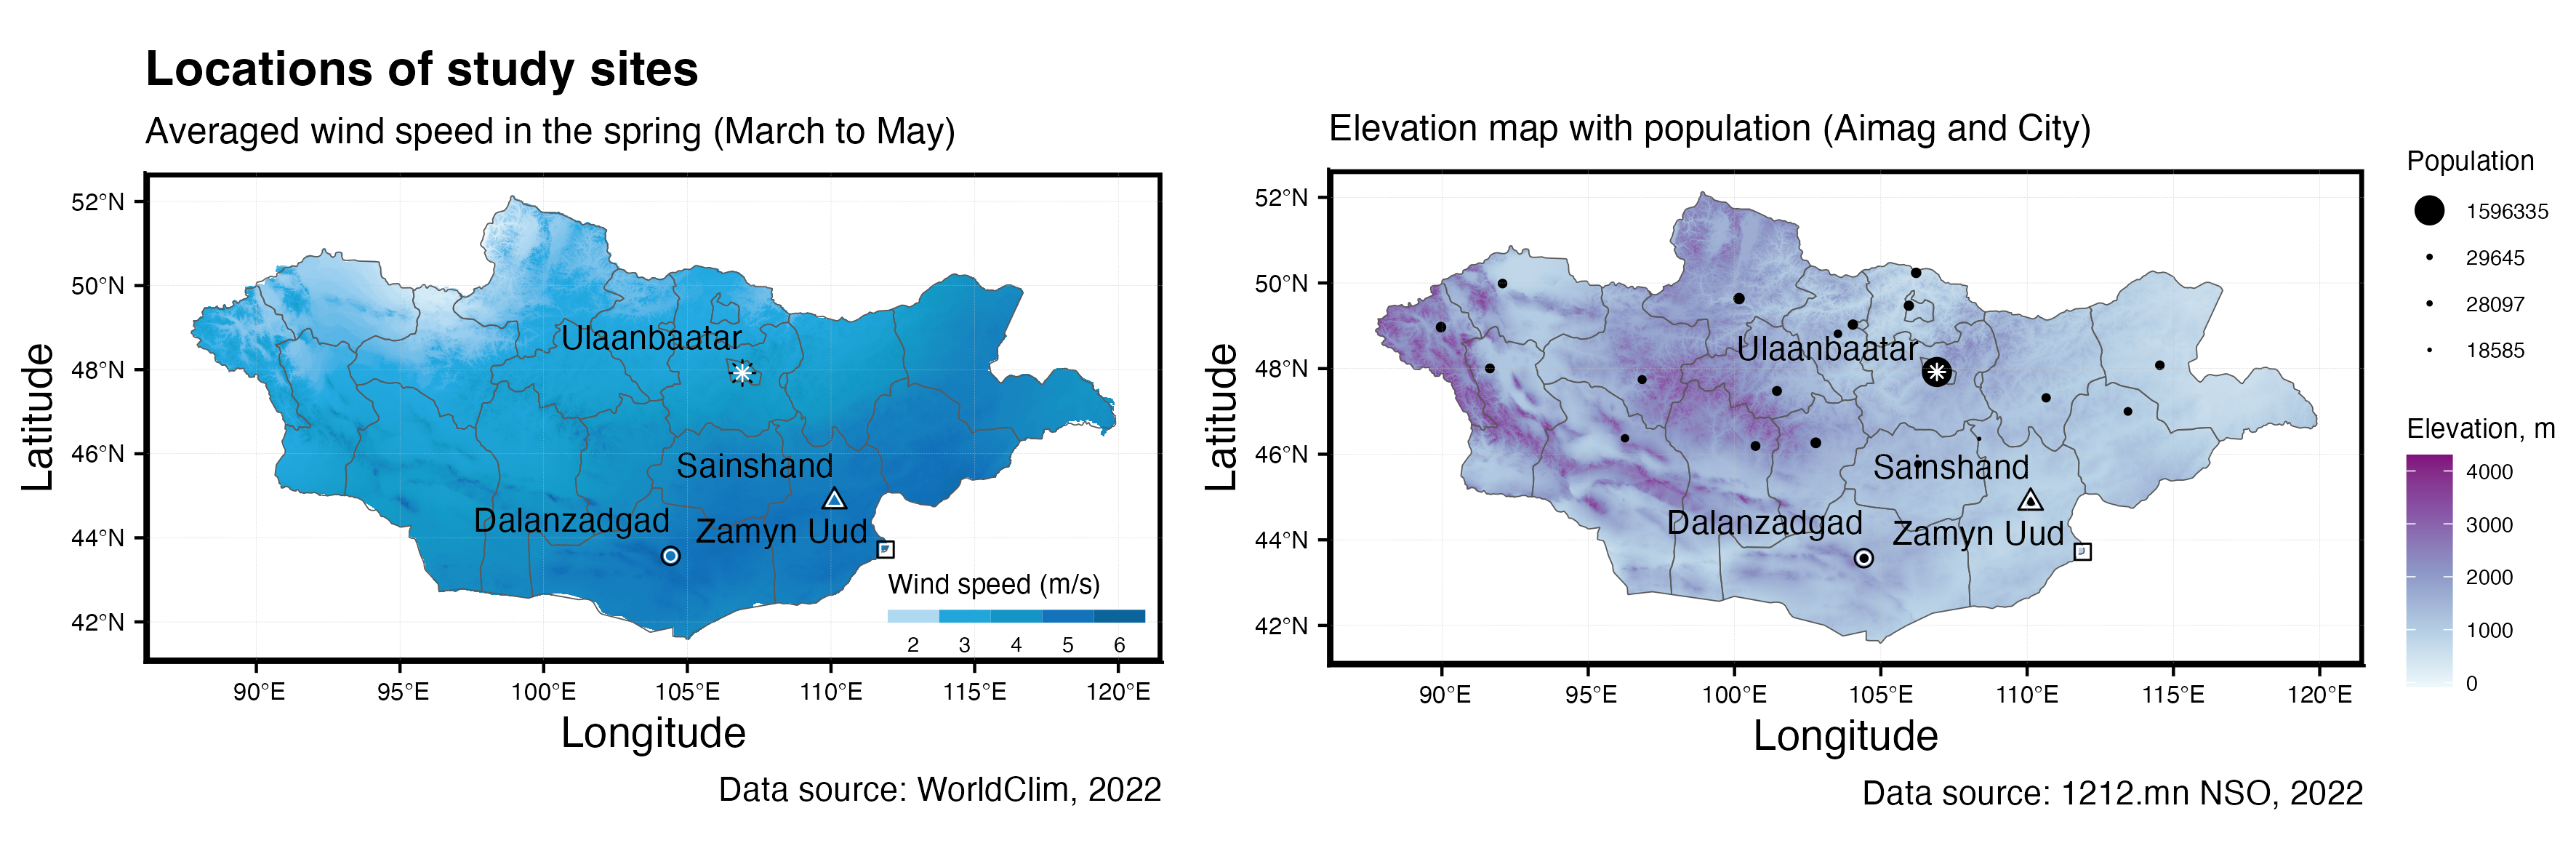
\includegraphics{../Data/03_figures/fig-1_sites_of_NIES.png}

}

\caption{\label{fig-1}Study sites}

\end{figure}%

\subsection{Study data and data
analysis}\label{study-data-and-data-analysis}

\subsubsection{Data}\label{data}

Particulate matter with aerodynamic diameters less than 2.5 \(\mu m\)
(PM2.5) and 10 \(\mu m\) (PM10) were measured at these sites using an
instrument that measures light scattering by air- borne particulates.
Meteorological parameters, including wind speed, wind direction and
visibility were determined by automatic instruments and are detailed in
previous articles (Jugder et al., 2011, 2012; Nishikawa, Sugimoto). The
instruments for measuring particulate matters were placed 2.0 m above
the ground level (AGL) at Dalanzadgad, Sainshand and Zamyn-Uud
(Table~\ref{tbl-1}). Wind sensors and visibility (meteorological optical
range-MOR) sensors with a maximum measurement range of 20 km were
installed at a height of 3 m AGL at the three Gobi sites. At the
Ulaanbaatar site, the wind sensor height and a visibility sensor was
placed at 15 m AGL.

\begin{table}

\caption{\label{tbl-1}Data}

\centering{

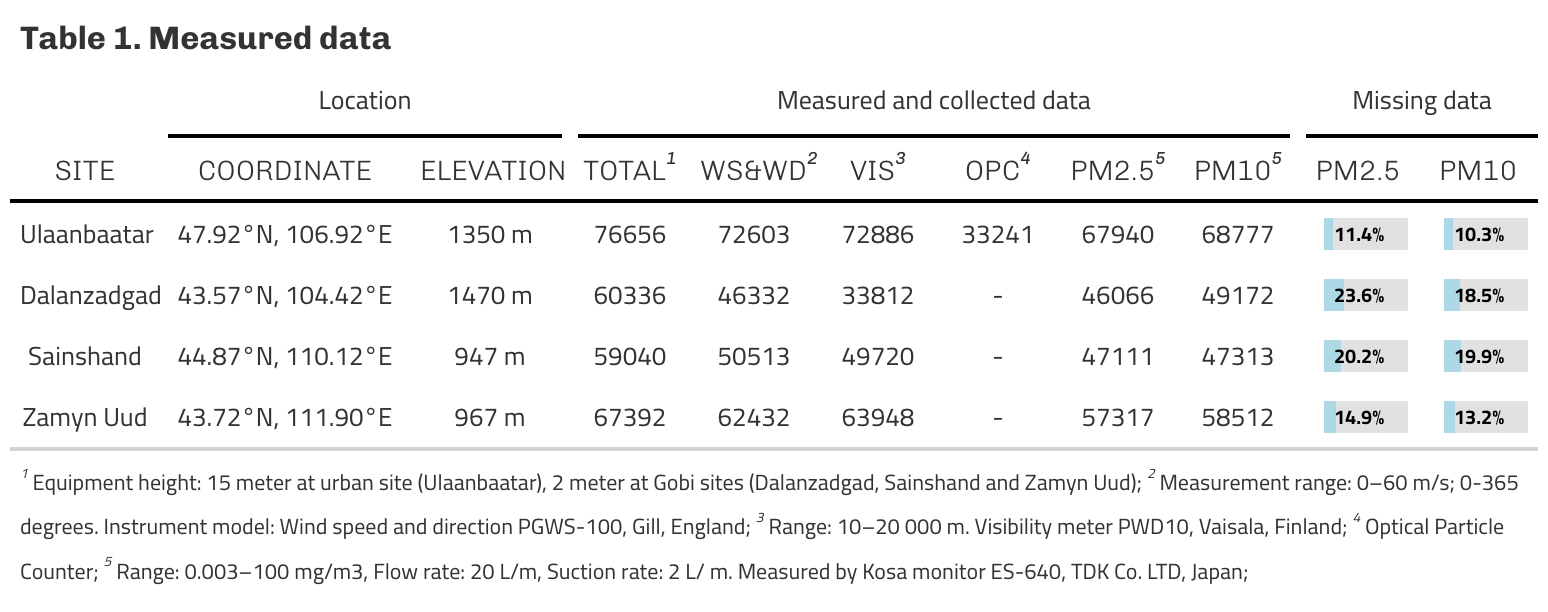
\includegraphics{../Data/03_tables/table-1_data_NIES.png}

}

\end{table}%

\subsubsection{Datasets}\label{datasets}

Datasets were obtained from measurements at Dalanzadgad, Sainshand, and
Zamyn-Uud from January 2009 to May 2018, and at Ulaanbaatar from the end
of April to May 2008. The data used in the study are based on hourly
means derived from 1 and 10 min averages. Additionally, the WMO defines
dust storms and sandstorms (dust events) as `'An ensemble of particles
of dust and sand energetically lifted to great heights by a strong and
turbulent wind'' (WMO-No.~407) and reducing visibility to less than 1000
m (WMO-No.~306). Therefore, data of wind speed, visibility, and dust
concentration were used in combination with synoptic weather
observations. Data sets comprise selected data collections from periods
of dust events, during which wind speeds and PM10 (PM2.5) concentration
rose dramatically and visibility dropped down considerably. Quantitative
criterion of wind speeds and dust con- centrations of PM10 for dust
events were explained in Section 2.2. Scalar mean wind speed and gust
winds were calculated from 1-s observations for the study
(EPA-454/R-99-005, 2000). The shorter averaging period wind is regarded
as the `'gust'' (Harper et al., 2010). The 3-s averages of wind speed
that are considered as gust wind speed (Harper et al., 2010), were used
in this study. Time series of number of days with dust events obtained
from synoptic weather observations at Dalanzadgad, Sainshand and
Zamyn-Uud during 1960--2012 were used.

We examined the PM data quality, and removed spikes those are above 7
\(mu m\), and when PM10,,. Due to electricity shortage and equipment
malfunctions contributed to the bad data, and missing data. In Sainshand
station, \ldots{} was \ldots{} Each stations has some features, we
treated each stations separately to remove suspective data.

At last, we filled the missing data using mtsdi R package (well-used for
time-series data), and improved the missing data percents by\ldots{}
from \ldots{} to \ldots{}

The MTSDI method (\citep{junger2003missing}, \citep{junger2012mtsdi})
uses the EM algorithm with the Autoregressive Integrated Moving Average
(ARIMA) method, also known as Box--Jenkins model (\citep{box2015time},
\citep{meyler1998forecasting}). The data provided by ARIMA (p, d, q)
depend on the number of autoregressive terms (p), the number of
differences (d), and the number of terms in the moving average (q)
(\citep{meyler1998forecasting}). Default configuration was used. The
mtdsi method is widely used to impute missing data like in cosmic data
\citep{fernandes2017data}. Similar multiple imputation methods have been
applied for multivariate solar data \citep{zhang2020solargan}, highly
univariate seasonal data even with the large amount of missing data
\citep{chaudhry2019method}, missin data imputation and modeling for
leaching processes \citep{he2017study}. Recently,
\citep{motesaddi2022effects} used the mtdsi method to imputing missing
data air pollution in Tehran (We used the complete data of temperature
(°C), relative humidity (RH) (\%), wind speed (m/s), barometric pressure
(BP) (mbar), PM10, PM2.5, NO2, CO, and CVD variables to impute SO2 and
O3 with the mtdsi R package.).

\begin{figure}

\centering{

\includegraphics{../Data/03_figures/fig-2_datasets_filled_by_mtdsi_NIES.png}

}

\caption{\label{fig-2}Extended PM datasets (red color presents the data
filled by mtdsi)}

\end{figure}%

\begin{figure}

\begin{minipage}{0.50\linewidth}

\centering{

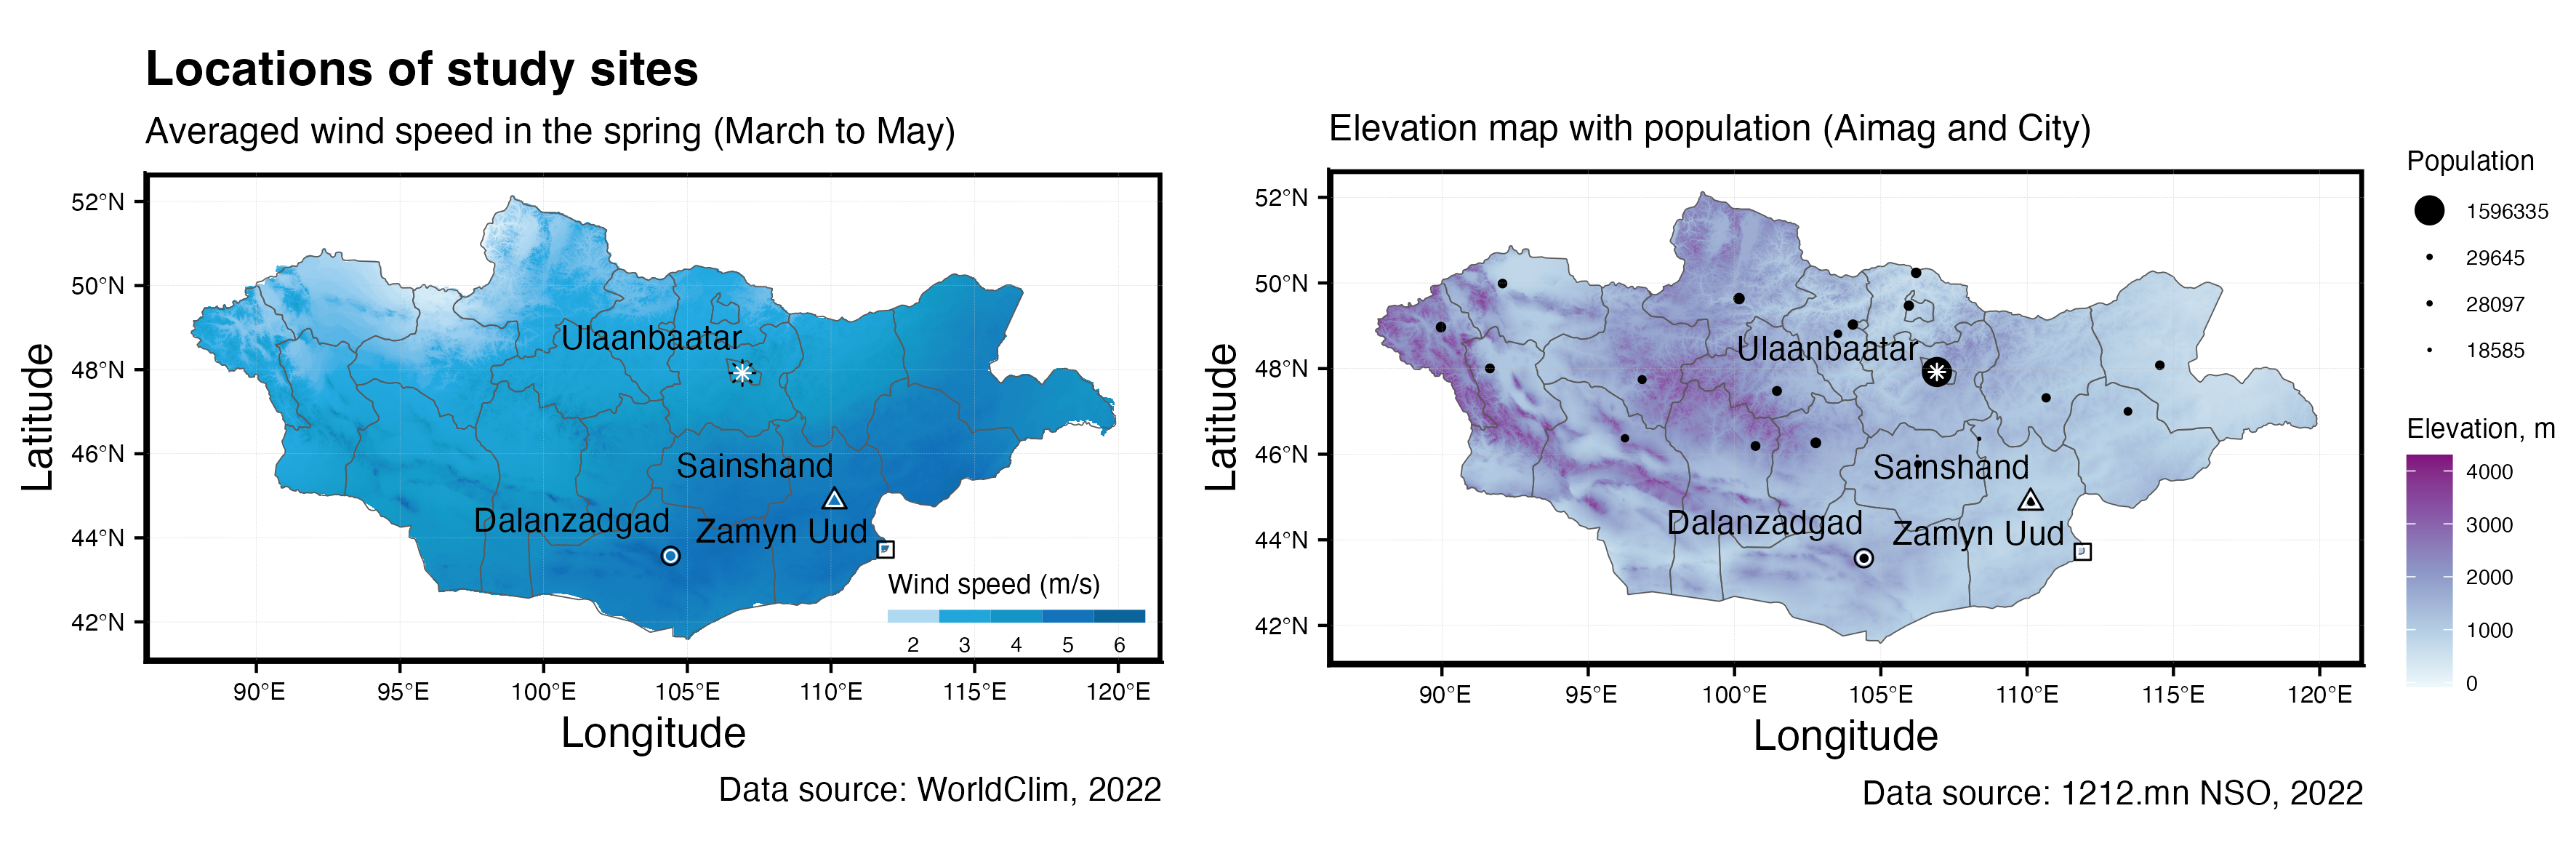
\includegraphics{../Data/03_figures/fig-1_sites_of_NIES.png}

}

\subcaption{\label{fig-surus}Surus}

\end{minipage}%
%
\begin{minipage}{0.50\linewidth}

\centering{

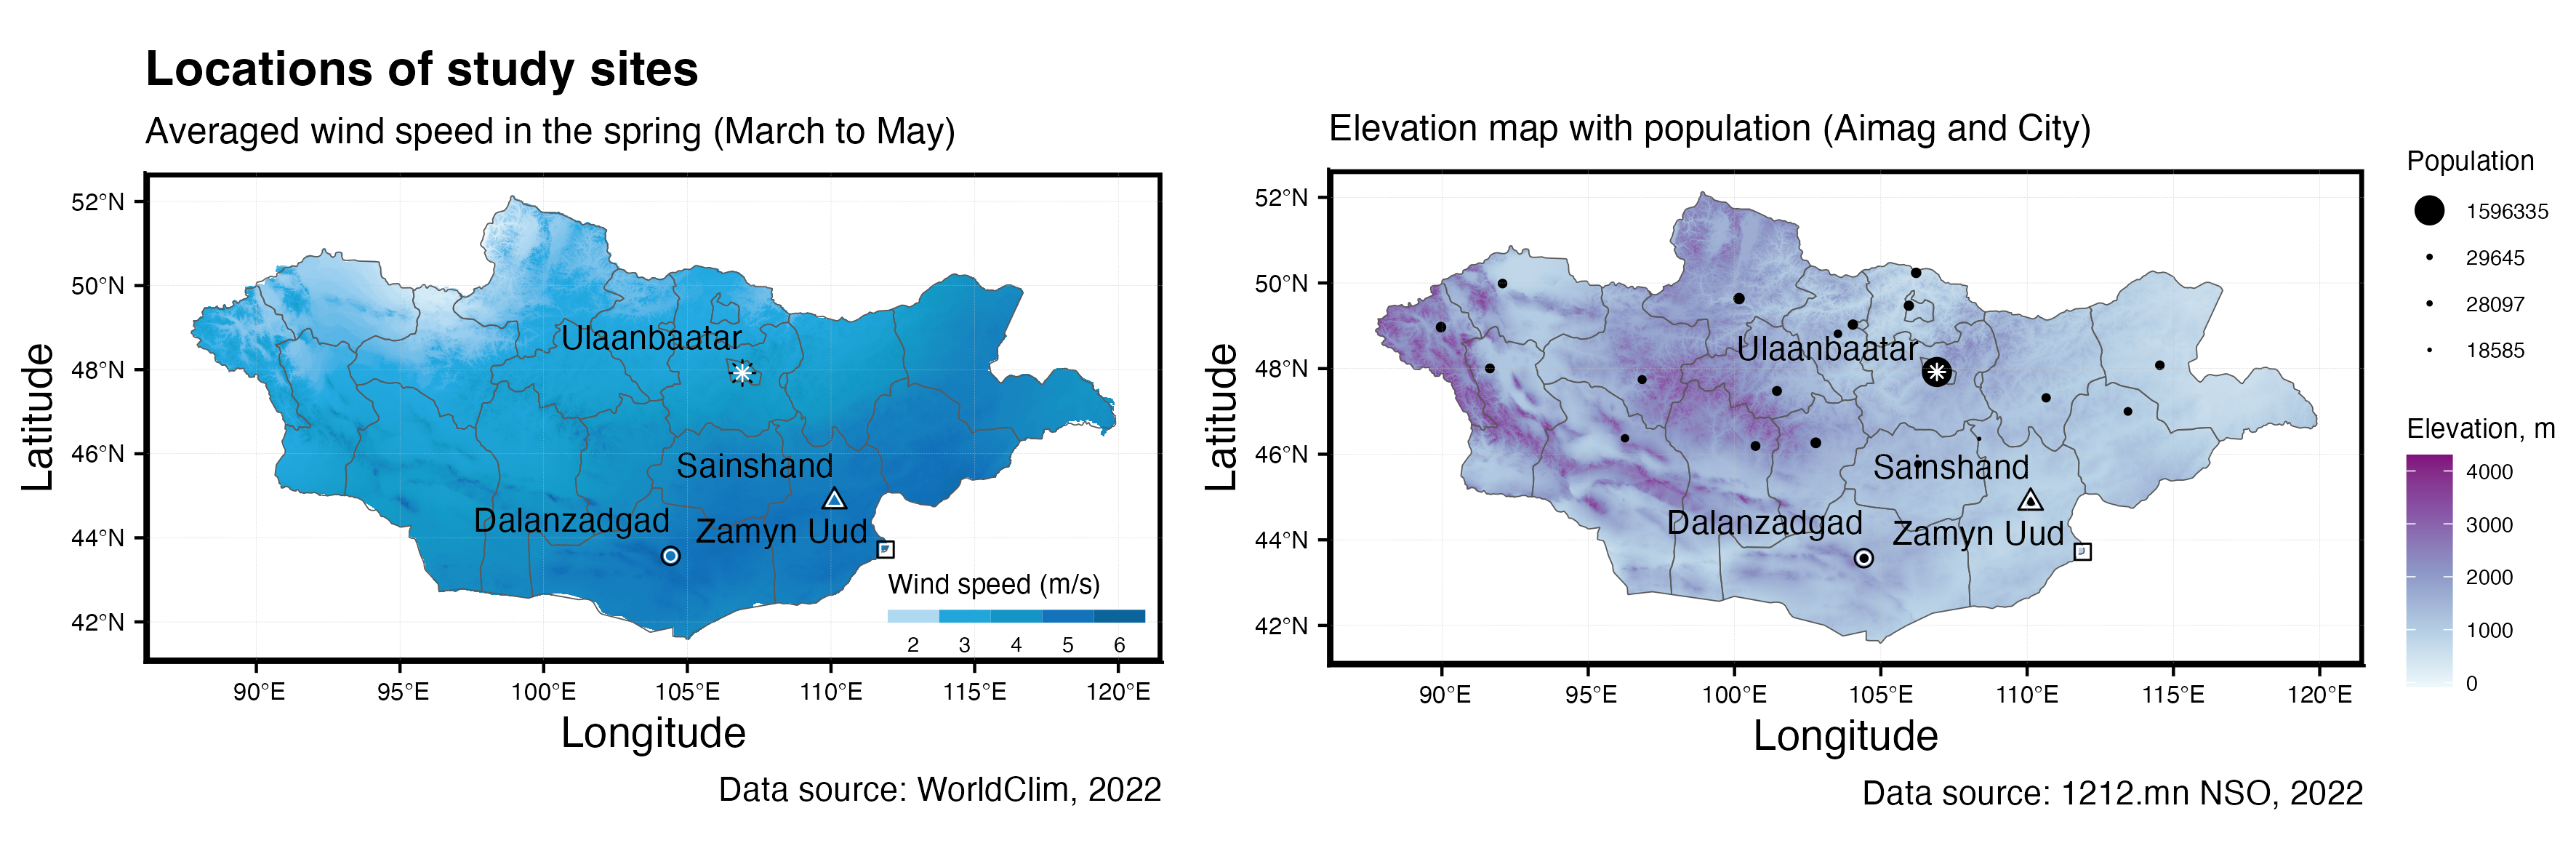
\includegraphics{../Data/03_figures/fig-1_sites_of_NIES.png}

}

\subcaption{\label{fig-hanno}Hanno}

\end{minipage}%

\caption{\label{fig-elephants}Famous Elephants}

\end{figure}%

\section{Results}\label{sec-results}

\subsection{Temporal variations}\label{temporal-variations}

To demonstrate the temporal variations of PM10/PM2.5: by illustrating
annual and seasonal changes from 2008 to 2020. a) Discuss the changes in
the seasonal maximums (peaks)

\begin{enumerate}
\def\labelenumi{\alph{enumi})}
\setcounter{enumi}{1}
\item
  Discuss the changes in duration of the dusty or polluted periods
\item
  Discuss the inter-annual variations
\end{enumerate}

\subsection{PM intercomparisons of sites between anthropogenic and
natural PM
sources}\label{pm-intercomparisons-of-sites-between-anthropogenic-and-natural-pm-sources}

To demonstrate the spatial variations of PM10/PM2.5: by illustrating
annual and seasonal changes from 2008 to 2020. a) Discuss the changes in
the seasonal maximums (peaks)

\begin{enumerate}
\def\labelenumi{\alph{enumi})}
\setcounter{enumi}{1}
\item
  Discuss the changes in duration of the dusty or polluted periods
\item
  Discuss the inter-site variations
\end{enumerate}

\section{Discussion}\label{sec-discussion}

\section{Conclusions}\label{sec-conclusions}

\textbf{Abstract:}

Air pollution, particularly particulate matter (PM), poses significant
health risks and environmental challenges globally. Mongolia, a country
characterized by diverse geographical features and climatic conditions,
experiences notable variations in PM2.5 and PM10 concentrations. This
manuscript explores the spatial and temporal patterns of PM2.5 and PM10
across Mongolia, identifying/delineating two distinct variations.
Utilizing extensive datasets and advanced analytical methods, this study
provides comprehensive insights into the dynamics of air quality in
Mongolia, which is crucial for formulating effective mitigation
strategies and policies.

\textbf{Introduction:}

Mongolia serves as a compelling case study for understanding the
complexities of air pollution dynamics. Despite its sparse population,
Mongolia faces severe air quality issues, particularly in urban centers
like Ulaanbaatar. The capital city experiences extreme winter pollution
episodes, earning it the dubious distinction of being one of the most
polluted cities globally. This dire situation stems from a unique blend
of factors, including rapid urbanization, inefficient heating practices,
and unfavorable meteorological conditions.

The impact of air pollution on public health cannot be overstated.
Exposure to elevated PM2.5 and PM10 levels is associated with
respiratory diseases, cardiovascular disorders, and even premature
mortality. Furthermore, air pollution poses a significant threat to
Mongolia's fragile ecosystems, exacerbating desertification and
contributing to biodiversity loss. Recognizing the urgency of addressing
this issue, this manuscript aims to dissect the spatial and temporal
variations of PM2.5 and PM10 concentrations in Mongolia, offering
insights essential for designing targeted interventions.

\subsection{This manuscript aims to elucidate the spatial and temporal
variations of PM2.5 and PM10 concentrations in Mongolia, shedding light
on the factors driving these
patterns.}\label{this-manuscript-aims-to-elucidate-the-spatial-and-temporal-variations-of-pm2.5-and-pm10-concentrations-in-mongolia-shedding-light-on-the-factors-driving-these-patterns.}

\subsection{Mongolia's unique geography, featuring vast steppes,
deserts, and mountain ranges, coupled with its climatic extremes,
results in complex patterns of air
pollution.}\label{mongolias-unique-geography-featuring-vast-steppes-deserts-and-mountain-ranges-coupled-with-its-climatic-extremes-results-in-complex-patterns-of-air-pollution.}

\textbf{Methods:}

This study employs a multifaceted approach to analyze PM2.5 and PM10
concentrations in Mongolia. Ground-based monitoring data from various
urban and rural sites are combined with satellite observations to
capture spatial variability. Sophisticated geospatial techniques,
including spatial interpolation and land use regression models, are
utilized to generate high-resolution maps of PM pollution across the
country. Temporal variations are examined through comprehensive
time-series analysis, considering seasonal trends, diurnal patterns, and
long-term trends. Additionally, meteorological parameters such as wind
speed, temperature inversions, and precipitation are integrated into the
analysis to elucidate their impact on PM levels.

This study employs a combination of ground-based monitoring data,
satellite observations, and meteorological datasets to analyze PM2.5 and
PM10 concentrations across Mongolia. Spatial analysis techniques,
including interpolation methods and geospatial modeling, are utilized to
map the distribution of PM pollution. Temporal variations are examined
through time-series analysis, considering seasonal and diurnal trends.
Additionally, meteorological parameters such as wind speed, temperature,
and precipitation are incorporated to understand their influence on PM
levels.

\textbf{Results:}

The analysis reveals two distinct spatial and temporal variations in
PM2.5 and PM10 concentrations across Mongolia. In the first pattern,
urban areas, especially the capital city Ulaanbaatar, exhibit
significantly higher PM levels compared to rural regions (Batmunkh et
al., 2020). This disparity is attributed to anthropogenic activities,
including residential heating, industrial emissions, and vehicular
traffic. Temporally, winter months coincide with peak pollution levels
in urban centers due to increased heating demand and temperature
inversions exacerbating pollutant accumulation (Dashdondog et al.,
2019).

Conversely, rural and remote areas display lower PM concentrations, with
seasonal variations influenced by factors such as dust storms,
wildfires, and agricultural practices (Battsengel et al., 2021). Spring
and summer elevated PM levels in these regions, primarily driven by dust
storms originating from arid landscapes and biomass burning activities.
Moreover, meteorological conditions, including wind patterns and
precipitation, play a crucial role in dispersing pollutants and shaping
temporal trends (Enkhbat et al., 2020).

\textbf{Discussion:}

The observed spatial and temporal variations in PM2.5 and PM10
concentrations underscore the intricate interplay between anthropogenic
and natural factors shaping air quality in Mongolia. While urban areas
grapple with pollution stemming from industrialization and urbanization,
rural regions contend with the impacts of climatic events such as dust
storms and wildfires. This stark dichotomy necessitates tailored
interventions that address the specific challenges faced by different
regions. Effective air quality management strategies must account for
these disparities, emphasizing targeted interventions tailored to
specific regions and seasons.

To combat air pollution effectively, holistic strategies integrating
regulatory measures, technological innovations, and public awareness
campaigns are imperative. In urban areas, transitioning to cleaner
heating technologies, improving public transportation infrastructure,
and enforcing emissions standards can significantly mitigate pollution
levels. In rural regions, initiatives focusing on sustainable land
management practices and early warning systems for dust storms and
wildfires are essential.

Furthermore, international collaboration and knowledge sharing can play
a pivotal role in addressing Mongolia's air quality challenges.
Leveraging expertise and resources from global partners can enhance
monitoring capabilities, foster innovation, and support
capacity-building efforts in air quality management.

\textbf{Conclusion:}

This manuscript highlights the complexity of air pollution dynamics in
Mongolia, characterized by two distinct spatial and temporal variations
in PM2.5 and PM10 concentrations.

Future work requires to : By elucidating the contributing factors and
underlying mechanisms driving these patterns, this study provides
valuable insights for policymakers, urban planners, and environmental
stakeholders. Addressing air quality challenges in Mongolia necessitates
multifaceted approaches that integrate regulatory measures,
technological innovations, and public awareness campaigns to safeguard
human health and ecological well-being.

\textbf{Keywords:} Air pollution, particulate matter, PM2.5, PM10,
spatial variation, temporal variation, Mongolia, urban pollution, rural
pollution, meteorological factors.

\citep{marrero2019} \# References \{.unnumbered\}

\{\#refs\}


  \bibliography{references.bib}


\end{document}
